\documentclass[a4paper]{report}
\usepackage[utf8]{inputenc}
\usepackage{amssymb}
\usepackage{amsmath}
\usepackage[margin=1in]{geometry}
\usepackage{graphicx}
\usepackage{verbatim}
\usepackage{bm}
\usepackage{listings}

\lstset{
  basicstyle=\ttfamily,
  mathescape
}

\title{Master Thesis Questions}
\author{André Oskar Andersen}
\date{}

\begin{document}
    
\maketitle

\section*{Teoretiske spørgsmål}
\begin{enumerate}
    \item Hvorfor bruger man heatmaps?
    \begin{quote}
        Heatmaps bruges til at modellere usikkerheden der er ved annoteringen
    \end{quote}
    \item Hvorfor bruger PCK en threshold baseret på torso height?
    \begin{quote}
        Det gør man for at inkorporere størrelsen af subjektet. Havde man fikset thresholden, havde predictionen været meget nemmere når personen er lille i billedet.
    \end{quote}
    \item Hvorfor kigger man på om afstanden ligger under en radius?
    \begin{quote}
        Ligesom ved årsagen til brugen af heatmaps, så modellerer thresholden usikkerheden der er ved annoteringen.
    \end{quote}
    \item Hvorfor gør du brug af MSE?
    \begin{quote}
        DeciWatch gør brug af en modificeret udgave af MSE. Unipose-LSTM gør brug af MSE. For at holde det konstant, valgte jeg bare at bruge MSE for alle modellerne.
    \end{quote}
    \item Hvad er fordelen ved at bruge ReLU?
    \begin{quote}
        Vigtigst af alt, lader det modellerne modellere ikke-lineære funktioner. Yderligere, så er der nogle andre fordelle, såsom (1) ReLU er hurtigt at udregne, (2) den afledte er nemt at udregne og (3) modsat andre activation functions såsom Sigmoid, har den en mindre sandsynlighed for at introducere vanishing gradientsa
    \end{quote}
    \item Hvorfor hjælper layer normalization
    \begin{quote}
        Ved at normalizere lagende af dataen undgår vi at inputtet ikke "ping-ponger" frem og tilbage, så dataen ikke pludseligt forskydes, idet den centrerer dataen. Dette burde sørge for, at færre epochs skal bruges.
        \begin{itemize}
            \item Batch normalization er svært at udregne for sekvenser med skiftende længder, små batches giver en dårlig representation (mean og std) for hele datasættet og batch normalization er dårlig til parallelisering.
            \item Input values in all neurons in the same layer are normalized for each data sample
            \item Gør træningen mere "stabil", ved at sørge for, at activation i forward og gradienterne i backpropegation ikke bliver for store 
            \item Input til et neuron er normalizeret (standardizeret) ved at anvende mean og std af neuronerne for dette lag 
        \end{itemize}
    \end{quote}
    \item Hvorfor gøres der brug af 1x1 convolutions
    \begin{quote}
        1x1 convolutions bruges som et fully-connected layer på tværs af filtrerne. Det bruges ofte til at downsample antallet af filtre.
    \end{quote}
    \item Hvorfor initializerer med Glorot?
    \begin{quote}
        Der er flere grunde til det. (1) vægtene hverken for store eller små, hvilket hjælper på vanishing/exploding gradients. (2) vi sørger for at der ikke er nogen symmetri, hvilket ville resultere i neuronerne have samme udregninger. 
    \end{quote}
    \item Kan du forklare cross-attention i en transformer?
    \begin{quote}
        Forskelligt fra self-attention hvor man kun arbejder med én sætning, så mixer cross-attention to sætninger (én fra encoder og én fra decoderen).
    \end{quote}
    \item Hvordan fungerer en convolution
    \begin{figure}[htbp]
        \centering
        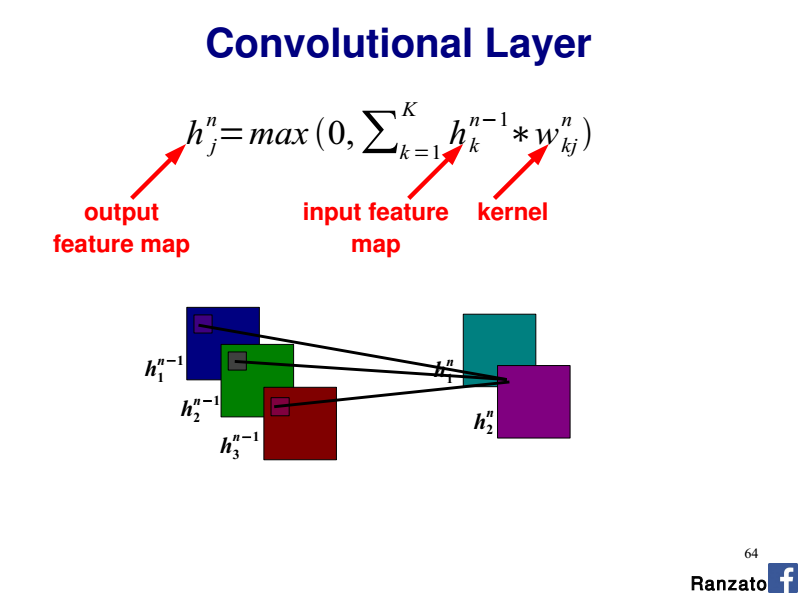
\includegraphics[width = 0.6 \textwidth]{./entities/convolutions_explained.png}
    \end{figure}
    \begin{quote}
        Hvert local receptive field i de $n$ input feature maps foldes (convolution) med dette feature maps tilknyttede kernel resultaterne af disse $n$ resultater lægges så sammen og placeres i output.
    \end{quote}
    \item Hvorfor bruger man positional encoding i transformeren?
    \begin{quote}
        Transformeren tager alle ordene på én gang som input, som så bliver processed samtidigt. Hvis vi ikke havde positional encoding ville positionen af ordene ikke blive brugt, men da denne information er vigtig, vælger man at bruge positional encoding.
    \end{quote}
    \item Hvad bruges self-attention til?
    \begin{quote}
        Self-attention bruges til at få modellen til at få en forståelse af context af ordene i sætningen.
    \end{quote}
    \item Hvad er målet med multi-head attention?
    \begin{quote}
        Ved hjælp af self-attention laver multi-head attention en meget kontekst-bevidst vector af input vector 
    \end{quote}
    \item Hvad er målet med skip-connections (residual connections)?
    \begin{quote}
        De bruges til at overkomme vanishing gradient
    \end{quote}
    \item Hvorfor bruger man look ahead masks in transformeren?
    \begin{quote}
        Hvis man ikke bruger dem, så har decoderen mulighed for at "se" de ord som den prøver at predicte. Look ahead mask bliver brugt ved at tilføje minus infinity til de ord som der ikke må ses
    \end{quote}
    \item Hvorfor bruger man padding mask i transformeren?
    \begin{quote}
        Det gør man for at sørge for, at modellen ikke lærer at "attend" til disse padding tokens.
    \end{quote}
    \item Hvad er ideen bag LSTMs?
    \begin{quote}
        En LSTM cell består af tre gates: (1) input-gate kontrollerer om ny information skal akkumuleres i cellen, (2) forget-gate kontrollerer om cellens hukommelse skal gensættes og (3) output-gate kontrollerer om cellens information skal sendes videre til den sidste state.
    \end{quote}
\end{enumerate}


\section*{Thesis-based spørgsmål}
\begin{enumerate}
    \item Hvilke andre metoder kunne man bruge?
    \item Du siger at du har introduceret noget evaluation bias i pretraining, da forskellige frames fra den samme video sequence kan optræde i forskellige subsets og den samme person derved optræder påtværs af subsets. Har du ikke samme problem i finetuning?
    \begin{quote}
        Både jo og nej. Jo, fordi den samme person kan optræde påtværs af subsets. Nej, fordi det er forskellige video sequences.
    \end{quote}
    \item Hvorfor er 3DConv den bedst performing model?
    \begin{quote}
        Det er svært at svare på, da de andre modeller ikke ser ud til at overfitte, som ellers kunne være en forklaring
    \end{quote}
    \item Hvordan performer din deciwatch i forholdet til det fra artiklen?
    \begin{quote}
        Vores DeciWatch performer noget dårligere end den fra artiklen, som nok højst sandsynligt kan forklares af forskellen i dataen
    \end{quote}
    \item Hvilke andre metoder findes der til at undgå overfitting?
    \begin{quote}
        Data augmentation og at gøre modellerne mere simple
    \end{quote}
    \item Hvorfor brugte du ikke data augmentation?
    \begin{quote}
        Det kunne jeg godt have gjort, men jeg skal så være lidt påpasselig, da man nemt kan "ødelægge" datasættet, ved eksempelvis at rotere videoerne for meget.
    \end{quote}
    \item Hvorfor bruger DeciWatch ikke alle frames?
    \begin{quote}
        Da nærliggende frames indeholder overflødigt information, argumenteres der for, at modellen ikke behøver at kigge på alle frames.
    \end{quote}
    \item Hvorfor denoiser DeciWatch sit input?
    \begin{quote}
        Det er svært at recover frames, især hvis de samplede poses indeholder noget noise. 
    \end{quote}
    \item Hvorfor er fem frames det optimale valg? 
    \begin{quote}
        Skaberen af Unipose har undersøgt sammenhængen imellem Unipose's performance og antallet af frames. De kom frem til, at det var udnødvendigt at bruge mere end fem frames, da performancen plateuer efter fem frames. Dette kan selvfølgelig være anderledes i vores tilfælde.
    \end{quote}
    \item Hvorfor hjælper dine modeller ikke på PCK$0.2$?
    \begin{quote}
        Vi tror det skyldes, at de predicted keypoints af pose-detectoren der klassificeres som forkert, simpelthen er så forkerte, at de ikke kan redes af vores modeller.
    \end{quote}
    \item Hvorfor splitter du data'en forskelligt for pretraining og finetuning?
    \begin{quote}
        Set i bakspejl, så burde jeg nok have fulgt min fremgang i finetuning igennem hele opgaven, men jeg havde ikke tænkt over det tidligere. I pretraining tænkte jeg, at datasættet var så stort og der var så meget variance, at det ikke var nødvendigt at tage de forhold som jeg gjorde i finetuning.
    \end{quote}
    \item I 3DConv hvorfor valgte du at have en temporal-dybde på $T$-længde med $K$ filtrer og ikke omvendt?
    \begin{quote}
        Ved den nuværende løsning vil de lærte kernels bestå af vægte der lærer at vægte den temporale information. Omvendt ville de lære at vægte de forskellige led, hvilket ikke giver så meget mening
    \end{quote}
    \item I 3DConv, kunne du ikke bare have ét filter som du bruger til alle keypoints?
    \begin{quote}
        Nej, fordi nogle af keypointne er nok mere afhængig af de tidligere frames end andre.
    \end{quote}
    \item Har du andre teorier for hvorfor fingrene er de sværeste led?
    \begin{quote}
        Det kan også skyldes, at disse led er de mindste led og de derfor er svære for pose-detectoren at finde, hvilke så også går videre i vores modeller.
    \end{quote}
\end{enumerate}


\end{document}